\documentclass[conference]{IEEEtran}
\IEEEoverridecommandlockouts
\raggedbottom
\setlength{\parskip}{1em}
% The preceding line is only needed to identify funding in the first footnote. If that is unneeded, please comment it out.
\usepackage{cite}
\usepackage{float}
\usepackage{amsmath,amssymb,amsfonts}
\usepackage{graphicx}
\usepackage{algorithmic}
\usepackage{textcomp}
\usepackage{xcolor}
\def\BibTeX{{\rm B\kern-.05em{\sc i\kern-.025em b}\kern-.08em
    T\kern-.1667em\lower.7ex\hbox{E}\kern-.125emX}}



    \begin{document}

\title{Biological Internet of Things \\
        \large A review and study of hybrid biological IoT systems}

\author{\IEEEauthorblockN{ Ganapathi Naayagam }
\IEEEauthorblockA{\textit{School of Computer Science and Engineering} \\
\textit{Vellore Institute of Technology, Chennai}}
\and
\IEEEauthorblockN{ Yash Ulhas Ambre}
\IEEEauthorblockA{\textit{School of Computer Science and Engineering} \\
    \textit{Vellore Institute of Technology, Chennai}}

}
\maketitle

\begin{abstract}

Plant cells have intrinsic bioelectric signals to communicate with 
themselves regarding external stimuli, these signals can be harnessed 
and connected with digital devices for use in novel applications. 
Since plants are commonplace beings that are usually overlooked, especially
by intruders, plants that have been connected to digital devices can 
act as covert sensors within an IoT system surveilling important places 
such as warehouses for theft and taking necessary actions using other 
devices connected in the same system. The plants are capable of sensing
movement, touch , and light. Tactically placed plant sensors are 
indispensable to security as well as an sustainale aspect to the environment.
This paper explores the applications a digital-biological hybrid plant
based IoT system can be used in.

\end{abstract}

\begin{IEEEkeywords}
\textbf{Keywords:} Internet of things, biohybrid systems, cyborg botany, 
plant spikerbox, plant sensing.
\end{IEEEkeywords}

\section{Introduction}
    Over the past century human/mammal-computer interaction has seen leaps
    and bounds to the extent that thought based control of prosthetics and 
    even extraction of music from scanning brain signals is possible \cite{zotero-65} . 
    However a different kingdom of living beings can also be integrated with 
    modern computer systems - plants. Plants switch their ubiquity and
    simplicity can act as crucial living sensors and actuators, aiding in 
    various new activities. In this paper, the commonplace aspect of plants
    is exploited to architect a surveillance system. 
    
    In many surveillance cases, the existence of sensors lead to perpetrators
    directly targeting and compromising the sensor or camera. A more covert,
    and environmentally integrable system will be of extreme value. For this
    reason, we propose converting plants into covert sensors for use in 
    surveillance. Plant cells have intrinsic bioelectric signals to 
    communicate with themselves regarding external stimuli, These signals are
    harvested and connected with digital devices for use in various 
    applications. Plants that have been connected to digital devices can act
    as covert sensors within an IoT system, surveilling important places such
    as warehouses for theft and taking necessary actions using other devices
    connected in the same system. The plants are capable of sensing 
    movement, touch, and light. The plant signals are harvested using
    specialized signal processing units, which is then passed on to 
    conventional electronic apparatus for making decisions within the
    IoT system. Tactically placed plant sensors can be indispensable to
    security as well as an aesthetic aspect to the environment. Apart from 
    security aspects, certain gestures on the plants can be used for 
    interaction with the daily environment as well, and in the future
    integrate organic as well as digital entities for a truly inclusive and
    sophisticated internet of things, which will open new realms of data and
    interaction to explore.

    \subsection{Concept of operation}
    Intruders often target surveillance systems by detecting them using 
    their EM signature or if they are an activated sensor through 
    specialized devices. Plant based IoT systems combine the functionalit
    y of multiple devices without having to source expensive, intricate and breakable sensors.

    \begin{figure}[H]
        \begin{center}
            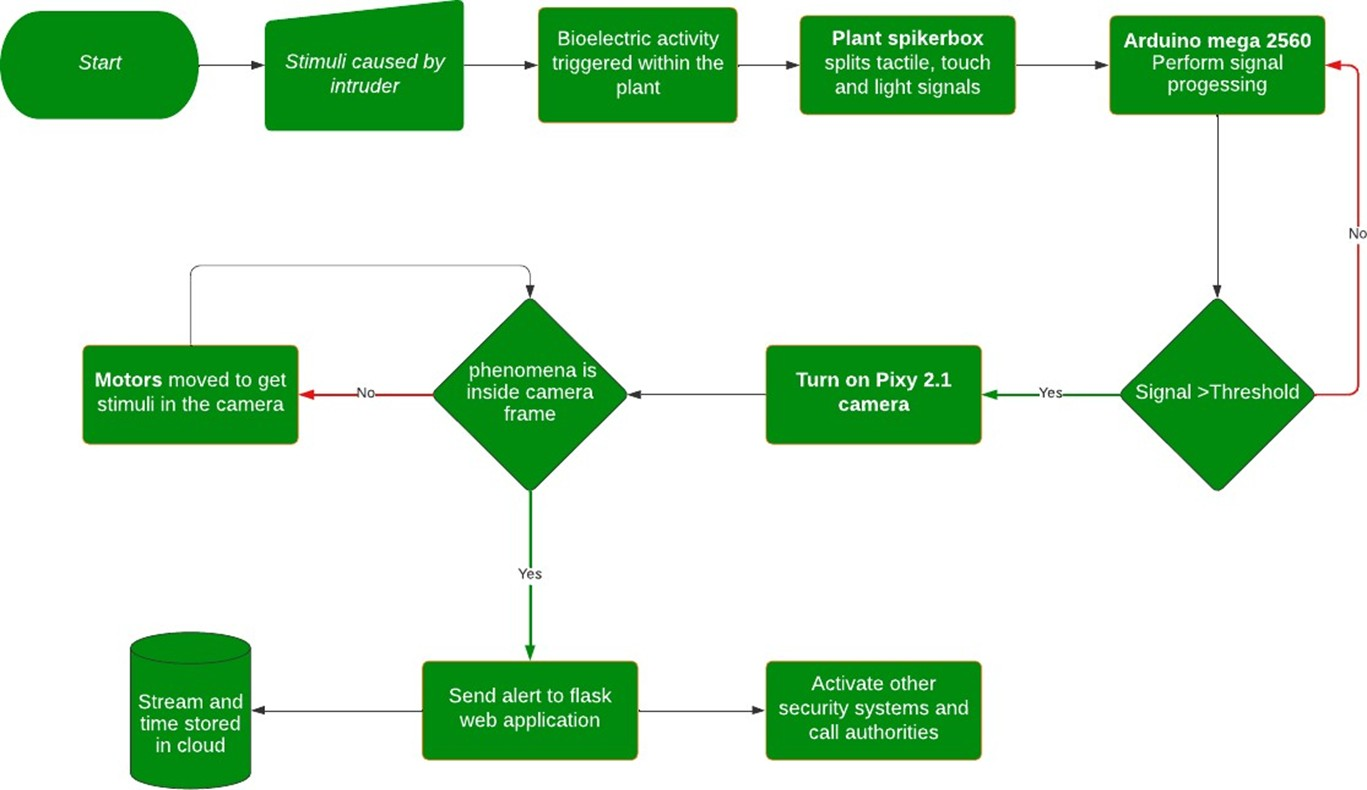
\includegraphics[width=0.47\textwidth]{flowchart}
        \end{center}
        \caption{Concept of system operation}\label{fig:}
    \end{figure}
    
    
    \subsection{Motivation}
    While this paper focuses on surveillance and detection of external 
    stimuli through plant signals, the project has scope in the future 
    to permeate more advanced applications. Given that vertical gardens, 
    smart farms and green city initiatives are seeing a boom, having 
    precise measurement and interconnection will allow for a more 
    connected and sophisticated world that better incorporates plant as
    well as animal life towards a more sustainable world. This is a
    pilot project to understand plant signals and measure them in 
    accordance with existing literature.

    In a sample operational situation, the plant detection system is 
    placed near a pathway an intruder must use to gain access to 
    different parts of their target. If an intruder passes by the
    plant's detection system, the plants will produce some electrical 
    signals which will be analyzed and processed. The plant has to be 
    capable of exhibiting a thigmonastic response, meaning it should 
    have a quick and active reaction to touch, sound or light and 
    physically respond/move must move to the same. This is important
    because the movement of the plant is caused by a potential difference
    and a corresponding spike, which is what is measured as a trigger 
    signal. Upon detection of the trigger signal, a hidden camera will
    be turned on and will track the anomaly/intrusion.

    This specific system will ensure that the intruder will not be aware
    that they are being tracked. Since the plants act as covert sensors 
    the factory officials will be alerted in no time. Furthermore, usage
    of plants is a sustainable and more supply chain friendly alternative
    as it is readily available and need not be imported in most countries.


    \subsection{Challenges}
    Some of the major challenges are that plant signals are very weak 
    since they are non-motorized, passive beings that do not generate 
    large electric or ionic potential differences. For this reason, even
    with sensitive electrodes, identifying and differentiating different
    signals is challenging. There are two major options to carry out data
    acquisition, invasive and non-invasive. Invasive method of signal 
    acquisition involves penetrating the epidermis of the plant using an
    electrode and reaching the core, while this promises high resolution
    , high amplitude signals, it might adversely affect the plant as 
    more signals are taken throughout the plant body over time. On the 
    other hand, a non-invasive method, while not promising in terms of
    acquiring signals, will be safer for the plant and more convenient 
    for experimentation. 


\section{Literature Review}

In the present, with existing issues such as global warming, it is clear
that a eco-conscious approach has to be taken to increasing interconnectivity
and interoperability in the advancement of IoT technology. On top of 
sustainability it is important to understand the underlying biology and 
better integrate artificial systems into existing biological systems for a more holistic
ecosystem. Plants have been known to have more than 15 senses, they are
stationary and have healing properties \cite{zotero-44}. These properties
make them ideal candidates to study the usage of a biohybrid IoT system.
 
Furthermore, movements such as industry 4.0 push for a varied and
decentralized set of sensors and actuators connected through the
cloud, however raw material restrictions and supply chain shortages
make this a cumbersome and painstaking process \cite{dadashpour2022}. 
The ubiquity of plants and their various capabilities will counteract
the problem with traditional sensors.

Integration of hybrid sensor based plants into the human environment encourage
better human-environment interaction \cite{holstius2004}. This study made a
living and robotic plants as markers in the environment to encourage recycling
and better the aesthetic of the location. This study involved two discrete 
open loop systems sparsely interacting with each other. The plant was not completely
connected with the robotics sensors, but the plant acted as the actuator, moving towards
the recyclables. In our study we would like to utilize plants' sensing capabilites,
hence further literature was expored.

Existing plant-electronics hybrid sensing projects involve injecting the 
plants with highly conductive electrodes, then sensing them using
another set of extrinsic electrodes 
Plant signals in this case are very clear and can be processed without
sophisticated signal processing tools. It can be used as an interface for
interaction with digital devices. The intrinsic conduction fluidic
polymer electrodes used were PEDOT - poly(3,4-ethylenedioxythiophene).
The plant is placed in a PEDOT solution, and the solution is allowed to 
penetrate the plant xylem, which now conducts all of the intrinsic plant
biosignals. The extrinsic electrode must be placed such that it is in 
contact with the intrinsic conductive polymer. The problem with this 
approach is that the polymer might interfere with the plant’s intrinsic
functions and furthermore, it is not a permanent solution. The polymer 
electrode eventually gets broken up, hence an open circuit is made inside
the plant, making any reading unreliable \cite{sareen2019}. 

One alternative to the chemical embedding approach is using optical nanosensors
and having the plant absorb them \cite{lew2020}. This approach makes the 
system completely self powered and does not involve any external power source.
FUrthermore there are no problems with continuity or circuit breakage causing
obscelesence in the future. This approach involved allowing plants to absorb 
nanosensors, then using a laser analyzer and observing the emission spectrum from
plants. This specific study designed and utilized nanosensors that detected arsenic
in the soil. This approach, however, is more expensive and too specialized, each
type of data to be collected involves a different nanosensor to be designed.


Easterly, D. Bio-Fi: Inverse Biotelemetry Projects. In the Proc of the 
12th annual ACM international conference on Multimedia. Spore is a 
self-sustaining ecosystem to visualize flow of stock prices. These works
utilize only the function that converts environmental energies into 
plants’ behavior. This paper involves use of electrodes as well as
actuators to influence the ecosystem. 

The most appropriate approaches found for our study were by \cite{easterly2004},
\cite{kuribayashi2007} and \cite{oezkaya2020}. Each of these approaches used
a combination of non invasive external electrodes and cheap, widely available 
sensors that rather then detecting the environment, detected the plants' biosignals
either using their own sensing rig or a commercially available system such as the plant
spikerbox \cite{zotero-53}. Each allowed the plant to sense and relay external information
such as stock pricing, light or movement. Studies also used plants that exhibited
rapid movement such as the Mimosa Pudica or the venus flytrap, which have the highest
biopotential difference from baseline. This careful selection of plants and external sensors
allow the avoidance of invasive chemicals, or unideal sensors. Hence, a similar approach was
adopted by ourselves. The plant spikerbox and Mimosa Pudica along with a portable computer
such as raspberry pi is ideal to the current paper.



\section{Requirements}
   \subsection{Hardware Requirements}
    \begin{itemize}
        \item Plant spikerbox: Spikerbox is used to separate, sense and preprocess the various signals from the plant by classifying each signal like proximity signal, touch signal etc.
        \item A laptop: To connect with the plant spikerbox for experimentation 
        \item Raspberry pi: To portably analyze the plant signals acquired from the spikerbox
        \item Pixy 2.1 camera: Performing cv operations and is used for tracking the people.
    \end{itemize} 

   \subsection{Software Requirements}
    \begin{itemize}
        \item Arduino software: This is the software used for Arduino programming
        \item Plant Spikerbox software: This is the software made by the spikerbox association to visualize and filter out the unnecessary signals from the plants.
        \item Pixymon: This is a software used to get the visual feedback from the pixycam and perform OpenCV operations on it.
    \end{itemize}

\section{Implementation and methodology} 

    The primary aspect of the implementation involves collecting plant
    biopotential signals through experimentation. The procedure for
    the same is outlined below.
    \subsection{Plant data collection}
    \vspace{-\baselineskip}
    For training the system and setting threshold a set of controlled
    experiments were conducted. The plant was placed in a dark room 
    approximately half hour after watering it. The following independent
    variables were used:
    \vspace{-\baselineskip}
    \begin{itemize}
        \item Light stimulus
        \item Wind stimulus
        \item touch stimulus
    \end{itemize}
    Light stimulus involves flashing a 50 lumen torch at the plant leaves.
    Wind stimulus involves using a hand fan to do 5 oscillations in the 
    direction of the plant. Touch stimulus involves using a plastic stick 
    to displace the respective plant stem by 1 cm.
    
    The above stimuli were carried out for 2 seconds continuously for a 
    set of 10 repetitions. Between each repetition, a 5 second gap is
    kept for differentiating between the signals.
    \begin{figure}[H]
        \begin{center}
        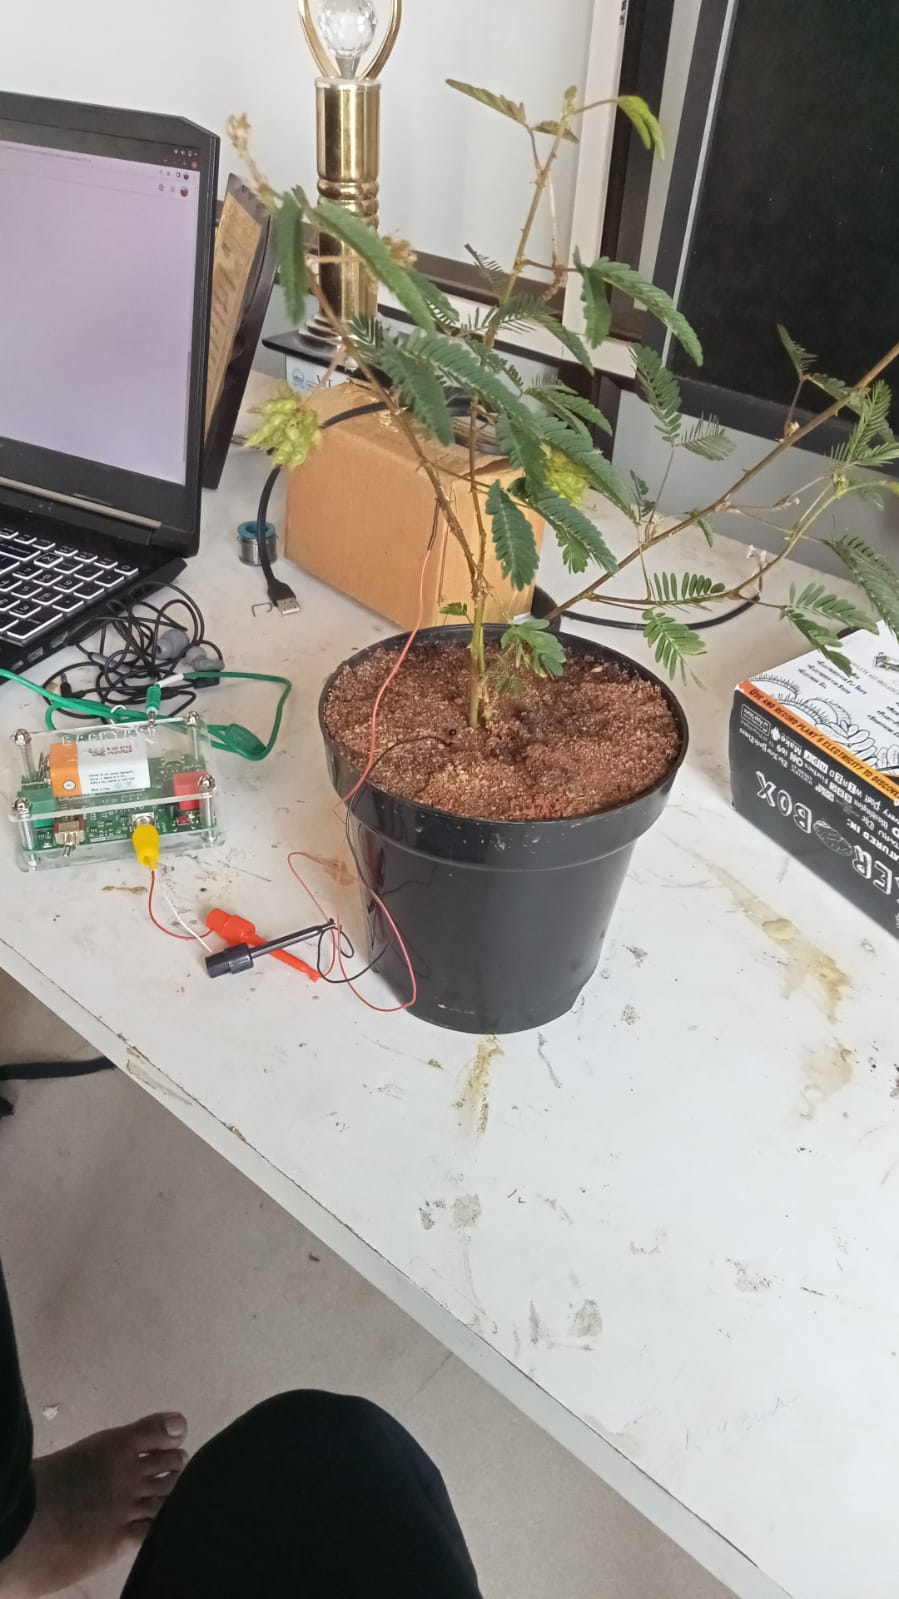
\includegraphics[trim={0 15cm 0 4cm},clip,width=0.4\textwidth]{spikesetup}
        \end{center}
        \caption{Setup of mimosa plant with spikerbox}\label{spikesetup}
    \end{figure}

    \vspace{-\baselineskip}

   
    In order to carry out the above actions, each component of the 
    plant spikerbox had to be effectively utilized.  
    \vspace{-\baselineskip}
    \begin{itemize}
        \item The spikerbox has several components, the main parts include:
        \item Electrodes - interfaces with the plant and collects signal
        \item Electrode connector clips - Conencts wires to PCB
        \item Signal jack - connect PCB to laptop for live viewing 
        \item Battery - allows portability and powers system
        \item spikerbox PCB - the actual amplifier and DAQ system
        \item conductive gel - improves signal collection
    \end{itemize}
    \begin{figure}[H]
        \begin{center}
            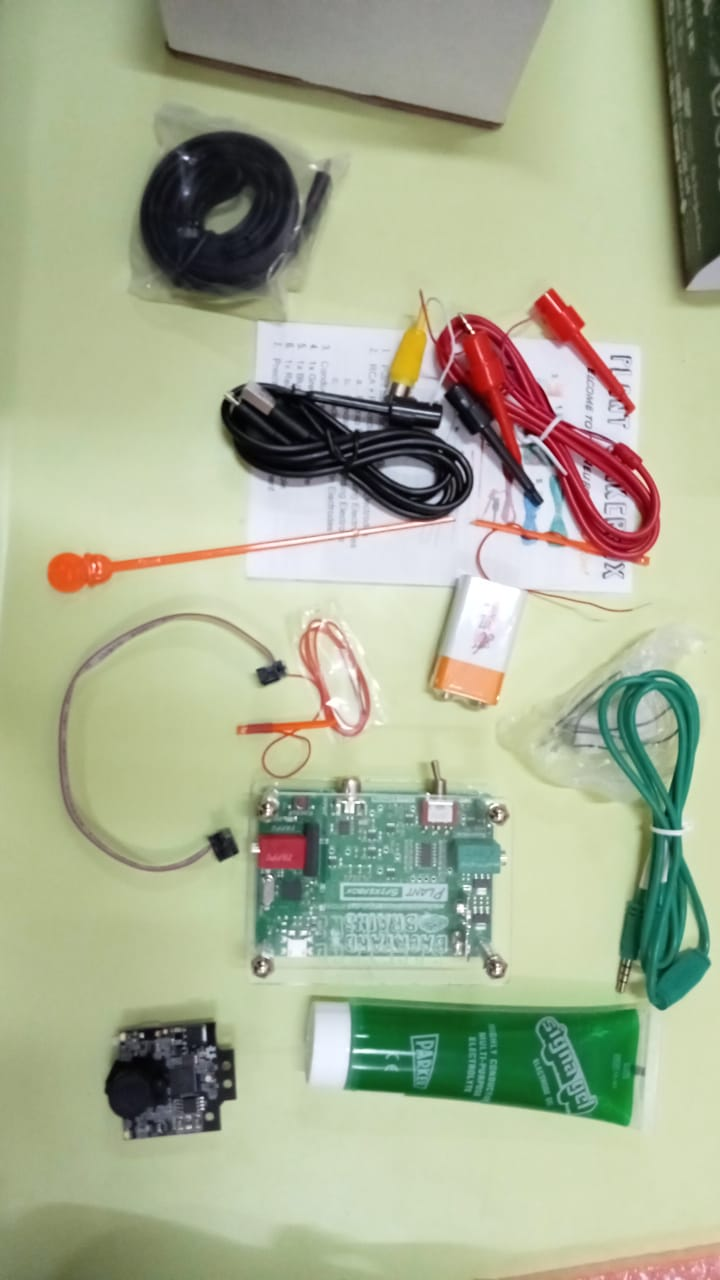
\includegraphics[width=0.27\textwidth,angle=90]{spikecomp}
        \end{center}
        \caption{All listed components of spikerbox}\label{spikecomp}
    \end{figure}
    
    Procedure to conduct experiment:
\begin{enumerate}
   \item  Connect red electrode to the plant by wrapping it around a joint on the plant
   \item  Place 1 drop of conductive gel on the point where the electrode makes contact with the plant
   \item  Place the ground electrode pin on the soil next to the plant
   \item  Clip the red and black electrode wires to the electrode connectors
   \item  Plug in the electrode connector on the jack provided in the spikerbox
   \item  Connect the green signal jack to the spikerbox and another device of choice(in this case a mobile phone was used)
   \item  Place 9V battery in the box’s power port and connect it
   \item  Flip the power switch to turn the spikerbox on
   \item  In the spike recorder application on the companion device, add the plant filter to only see the plant signals
\end{enumerate}

\section{Results and discussion}

Spikes detected from spikerbox:

As previously mentioned, three sets of experiments with three stimuli 
were carried out. The figures ~\ref{fig:light}, ~\ref{fig:wind}, ~\ref{fig:touch} 
below illustrate the data collected with the 3 stimuli.

\begin{figure}[H]
    \begin{center}
        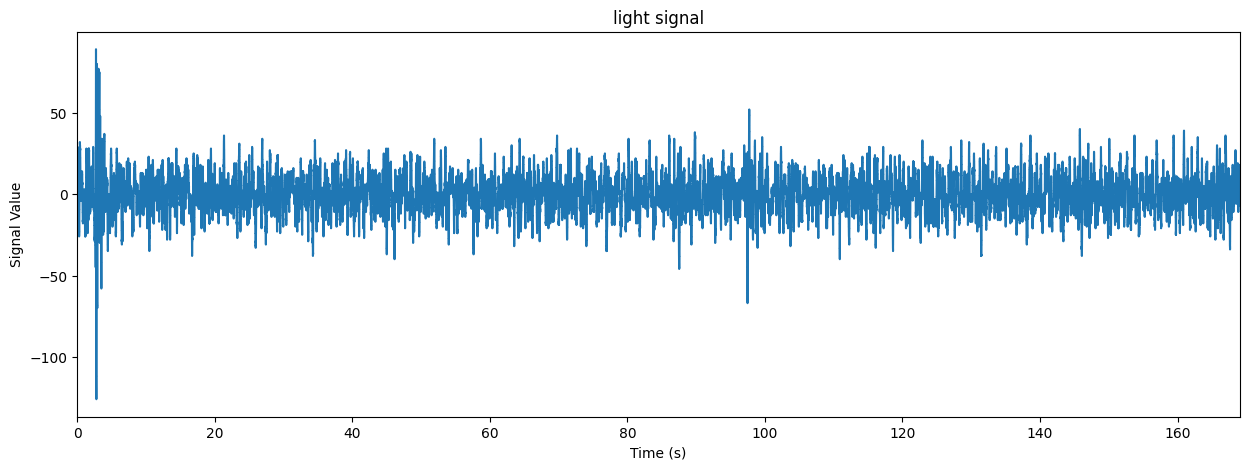
\includegraphics[width=0.48\textwidth]{light}
    \end{center}
    \vspace{-\baselineskip}
    \caption{Spikerbox data of Mimosa reaction to light stimuli}\label{fig:light}
\end{figure}

\begin{figure}[H]
    \begin{center}
        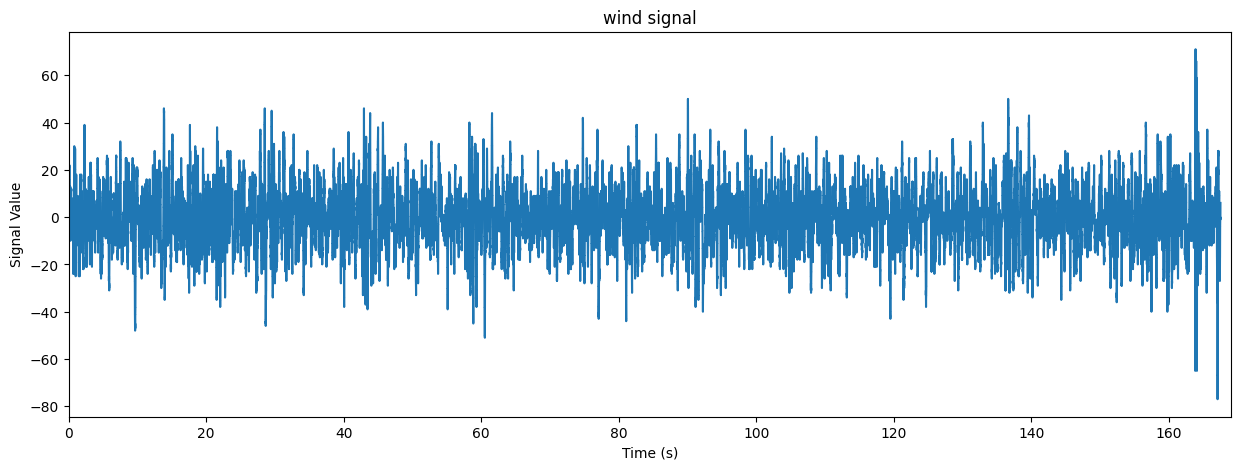
\includegraphics[width=0.48\textwidth]{wind}
    \end{center}
    \vspace{-\baselineskip}
    \caption{Spikerbox data of Mimosa reaction to wind stimuli}\label{fig:wind}
\end{figure}

\begin{figure}[H]
    \begin{center}
        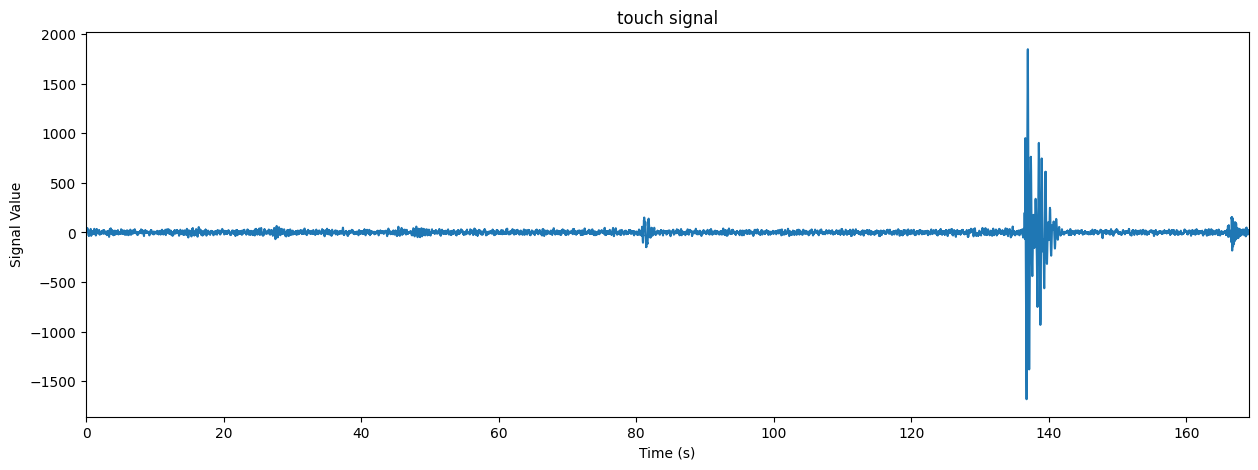
\includegraphics[width=0.48\textwidth]{touch}
    \end{center}
    \vspace{-\baselineskip}
    \caption{Spikerbox data of Mimosa reaction to touch stimuli}\label{fig:touch}
\end{figure}


In the generated graphs, there is no discernible difference between 
ambient noise, burst noises and signals that were supposed to have been 
generated. In order to find this a low pass filter with the threshold as 
15 hertz was used, since the backyard brains website suggested that plant
signals are in the lowest 1-10 range. 

This approach, however, led to the graph completely flat-lining. Therefore
,an alternative method was tried. MFCC conversion was a method utilized for
plant hybrid signal filtering and processing \cite{duerr2020}. MFCC is a feature extraction 
method where sinusoidal components of waves are represented as coefficients.

This signal and noise can be discrete. It involves selecting a window
size, setting a frame length and then finding the discrete fourier
transform of the signal and finally triangular filter banks are applied, 
upon which the final heatmap of the signals can be retrieved. Generally, 
at the end just the signals must be noticeable in the heatmap, however
when applied for the data acquired through the spikerbox, the entire 
length of recording was marked high in the final MFCC heatmap

The electronics aspects of the BIoT system worked as shown in Fig.~\ref{fig:obj} and Fig.~\ref{pixy}.
\begin{figure}[H]
    \begin{center}
        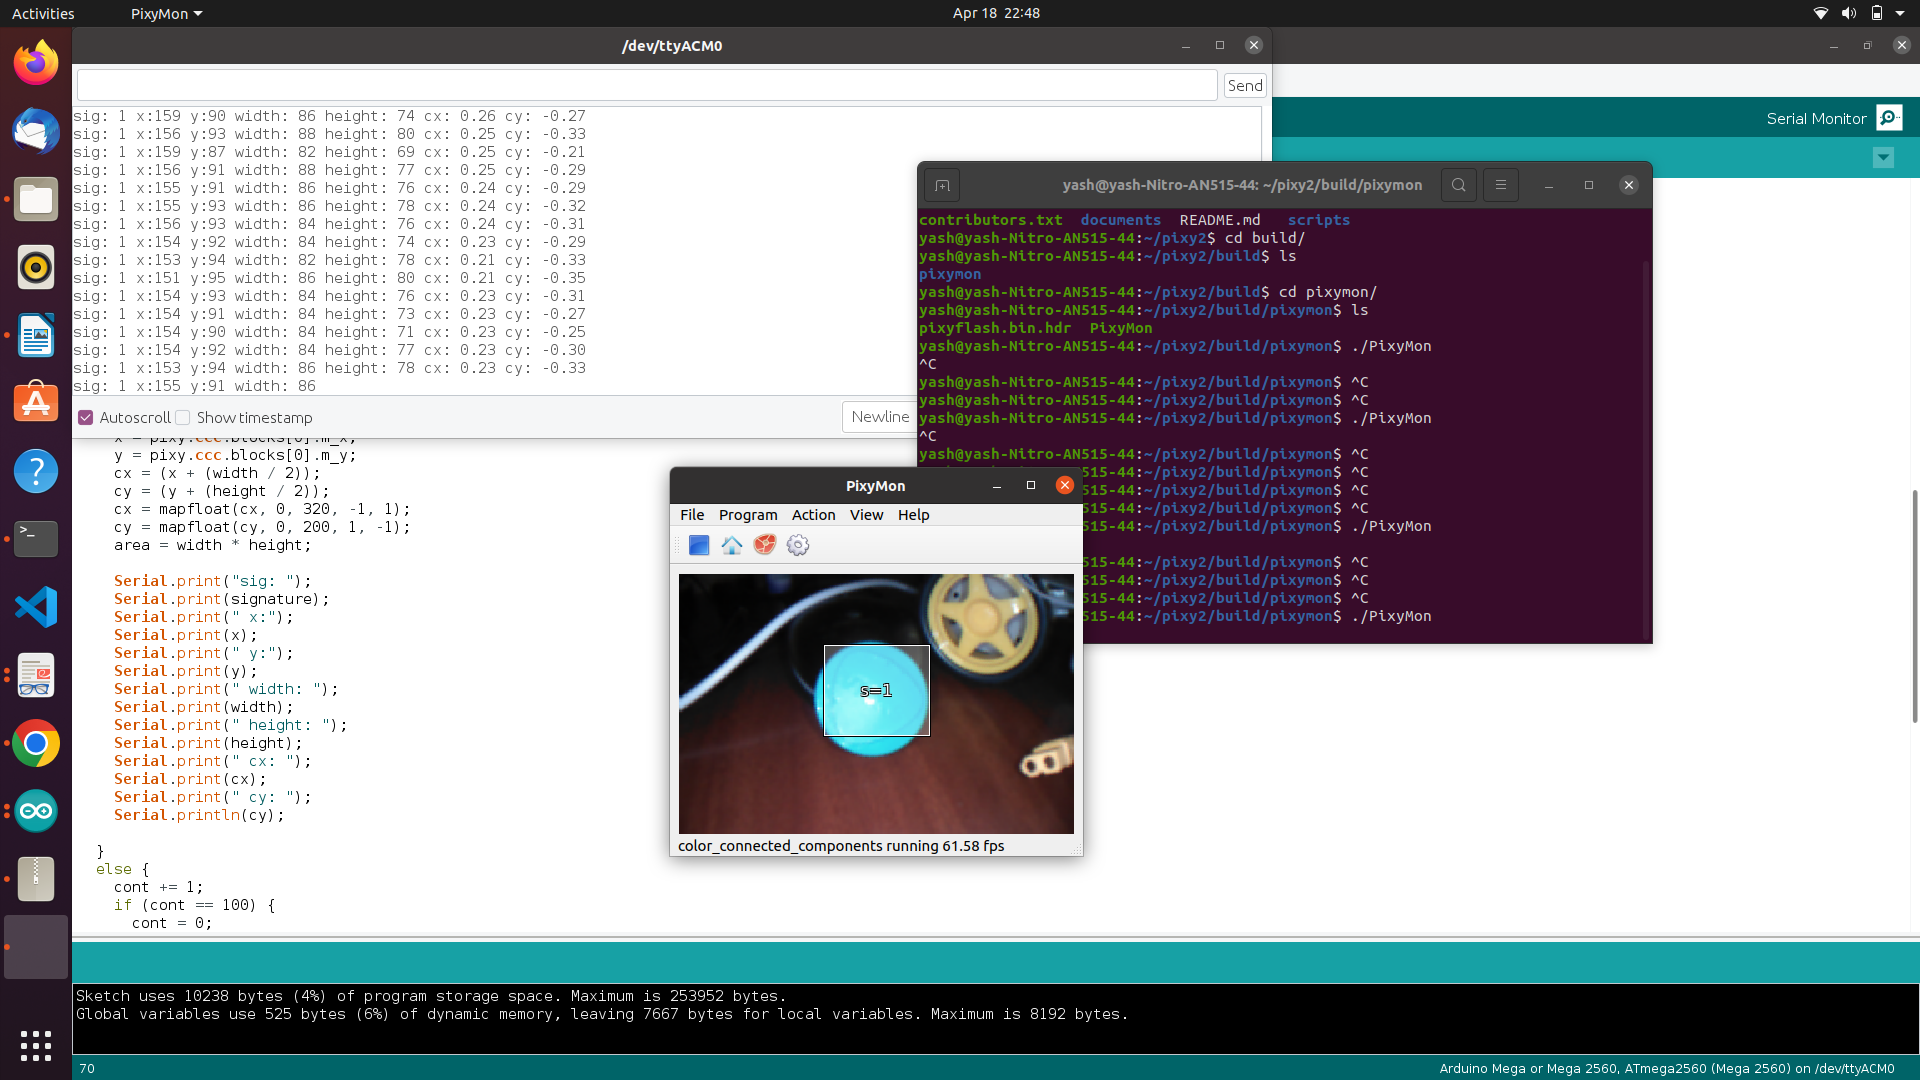
\includegraphics[width=0.47\textwidth]{objdet}
    \end{center}
    \caption{Screenshot of Object detection from camera}\label{fig:obj}
\end{figure}

\begin{figure}[H]
    \begin{center}
        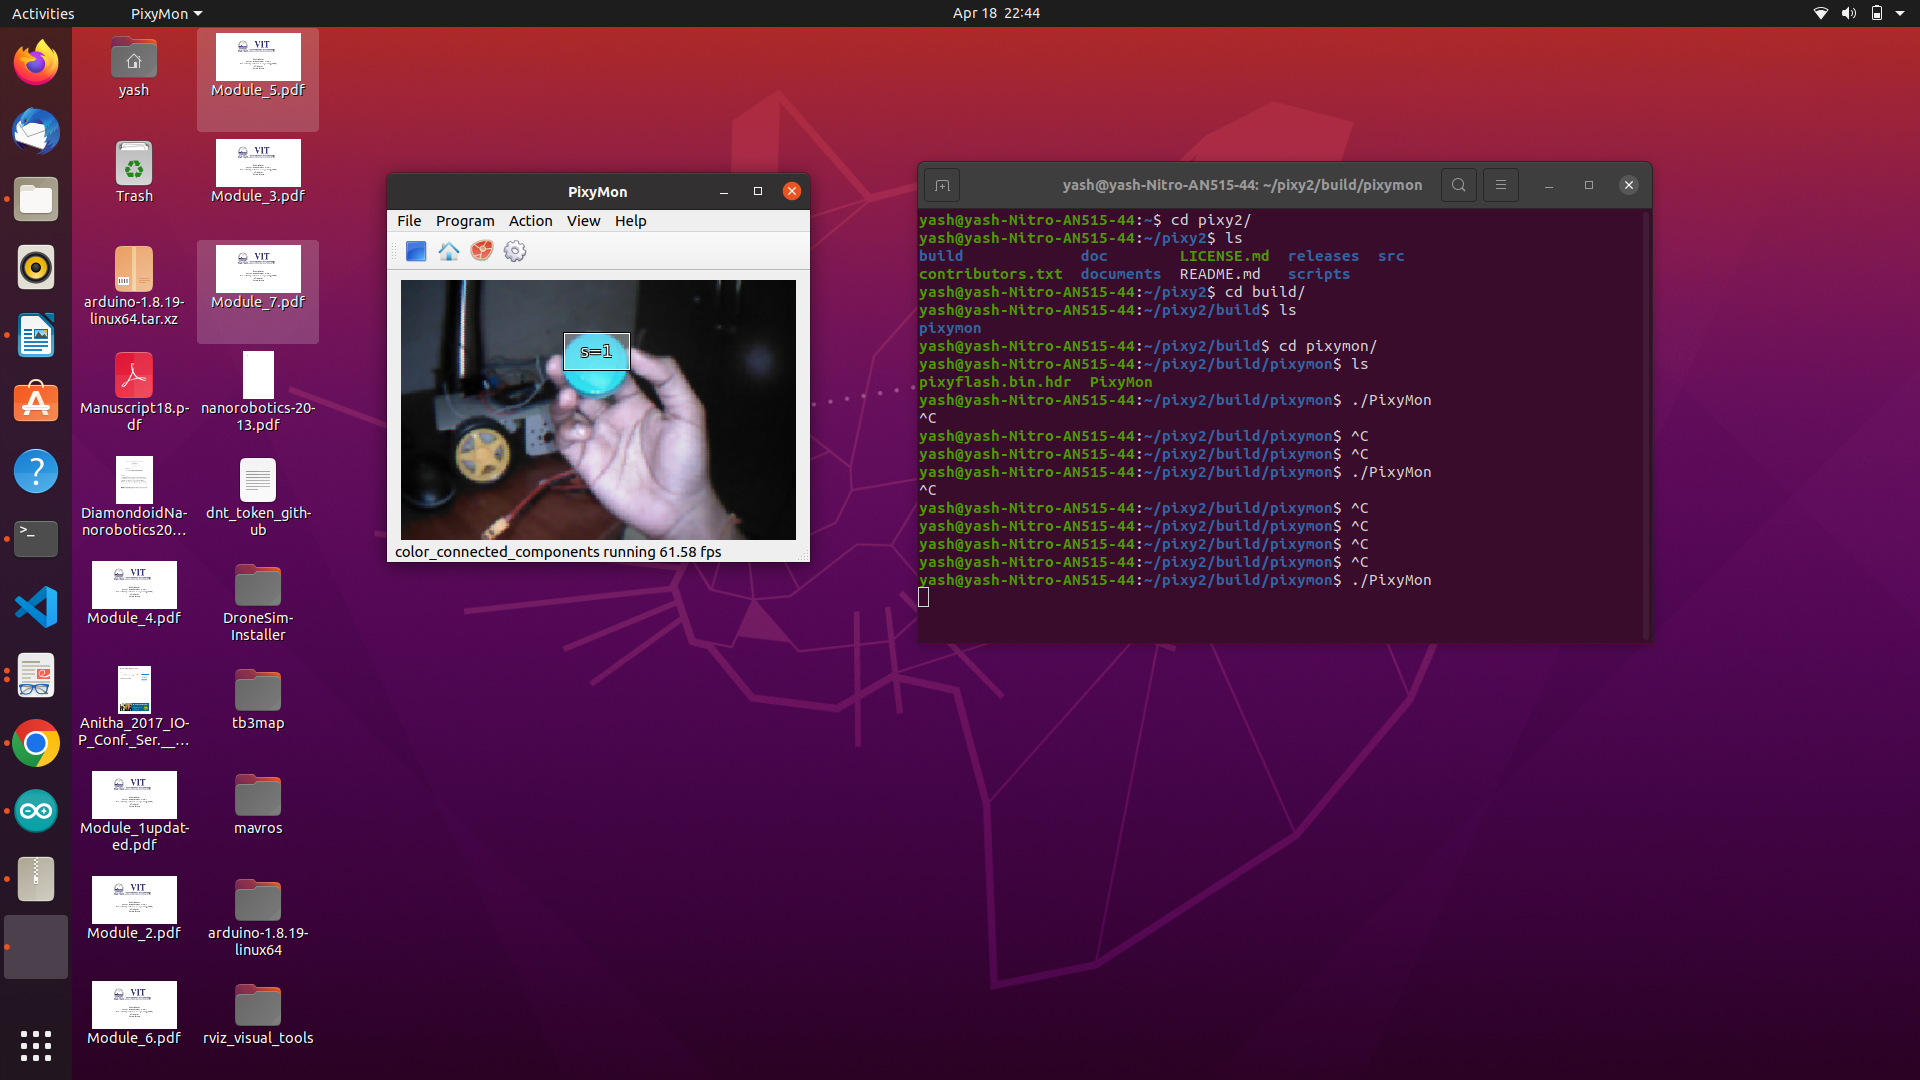
\includegraphics[width=0.47\textwidth]{pixy}
    \end{center}
    \caption{Screenshot of algorithm adding bounding box to detected object}\label{pixy}
\end{figure}


\section{Conclusion}
In conclusion, a thigmonastic plant such as Mimosa Pudica along with 
special amplifiers can act as multiple sensors and covert sensors in 
unique situations, hence acting as a low power sustainable IoT system.
The plant signals, however, for various types of signals are 
indistinguishable, a method to find and differentiate these signals
will truly unlock the potential of this specific device. 



\section*{Acknowledgment}

We wish to express our sincere thanks and deep sense of gratitude to our 
project guide, Prof. Dr. Rekha D., School of Computer Science and Engineering,
Vellore Institute of Technology, Chennai, for her consistent encouragement
and valuable guidance offered to us in a pleasant manner throughout the 
course of the project work. 

We are extremely grateful to Dr. Ganesan R, Dean of School of Computer 
Science and Engineering, VIT Chennai, for extending the facilities of the 
School towards our project and for her unstinting support. 

We also take this opportunity to thank all the faculty of the School for 
their support and their wisdom imparted to us throughout the course. We 
would like to thank all the lab assistants for helping us in our project. We thank our parents, family, and friends for bearing with us throughout the course of our project and for the opportunity they provided us in undergoing this course in such a prestigious institution.

%bib style was previously plain
    \bibliographystyle{unsrt}
    \bibliography{biot}

    \end{document}
